\documentclass[a4,a4paper]{article}

\input{~/mi-preamble-latex/mypreamble.tex}
 

\pagestyle{fancy}
\fancyhf{}
\chead{UTN Facultad Regional La Rioja - Esteban Bustamante}
\rhead{\includegraphics*[width=0.8cm]{/home/esbon1253/mi-preamble-latex/utnlogo.jpg}}
\cfoot{Anteproyecto de Trabajo Final}
\rfoot{\thepage}

\title{Anteproyecto de Trabajo Final \\ Firmware para un Decoder MPEG-2 prototipado en FPGA }
\author{Esteban Adriel Bustamante   \\ DNI: 436124923 \\ Legajo: 30-6567 \\ Profesor Titular: Ing. Pedro Chahín Rearte\\ Profesor: Ing. Oscar Almonacid\\ Tutor: Ing. Ricardo Maldonado}
\date{2025}


\begin{document}
\maketitle
\begin{center}
  \includegraphics[width=0.9\textwidth]{/home/esbon1253/mi-preamble-latex/utnlogo.jpg}
\linebreak
  UTN FACULTAD REGIONAL LA RIOJA
\end{center}

\pagebreak
\newpage

\tableofcontents

\pagebreak
\newpage
% Diagnóstico
% \section{Introducción}
% \label{sec:intro}
% Tal como fue sugerido por la cátedra, se utilizará la metodología \textit{5W + 1H} para el desarrollo del problema a ser resuelto en el trabajo final de la carrera. Debe ser dicho que si bien hay  un enfoque tanto innovador como pedagógico en el mismo, por sobre todo se busca explotar la capacidad de diseño de un sistema, de forma tal que se logre una solución realmente adecuada y eficiente. Es decir que no solo se buscará aprender y enseñar de forma anecdótica, sino realmente buscar la mejor opción para la solución del problema planteado, de igual forma que lo realizaría una empresa.

\section{Diagnóstico}
\label{sec:problema}
\par Se comienza por la descripción del problema haciendo uso del método de las 5W, para que de una forma clara podamos esclarecer cuál es la problemática a solucionar y en este caso, la necesidad a suplir.

\subsection{¿Qué?}
\label{sec:que}
El problema que se presenta en cuestión es el desarrollo de un firmware para un Decodificador MPEG-2 VLSI prototipado en FPGA, conforme con la norma ISO/IEC 13818-4, con un submuestreo 4:2:0. En la Figura\ref{fig:fig1} observamos el bloque completo. Es importante notar que la entrada es un bitstream  en formato MPEG-2 y la salida es RGB, es decir que se podría conectar la salida a un conector HDMI y visualizar un video entrante en alguna pantalla.


\begin{figure}[ht]
  \centering
  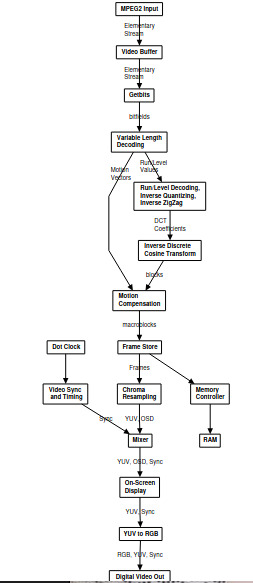
\includegraphics[width=0.3\textwidth]{figures/1.jpeg}
  \caption{\label{fig:fig1} Pipeline del Decoder MPEG-2}
\end{figure}

\pagebreak
\newpage

\subsection{¿Por qué?}
\label{sec:por-que}

El decodificador en sí no contiene en su arquitectura lazos de control ni tampoco tiene un microprocesador embebido que lo configure para su funcionamiento. Resulta crítico el desarrollo de un firmware robusto que permita controlar en tiempo real el bitstream del decodificador, y por supuesto que se encargue de la inicialización correcta del mismo, ya que en cualquier sistema que se piense para su integración el tráfico de bits no debe cortarse o en todo caso si se interrumpe su normal funcionamiento debiera claramente saberse el causante del error.

\subsection{¿Dónde?}
\label{sec:donde}

En todos los sistemas donde se utilizan aceleradores por hardware de sistemas de visión artificial, especialmente en este caso VLSI aplicable a dispositivos de bajo consumo de potencia como aquellos que funcionan a batería. Por ej, podríamos tener un Codec MPEG-2 por hardware en un Smartphone que pretenda tener reproducción de videos a una alta tasa de cuadros por segundo. Otra aplicación típica y actual  es en la televisión digital DVB, donde los receptores poseen decodificadores MPEG-2, y quien logra la mayor simplicidad cumpliendo la normativa establecida, logra acceder al mercado mas eficientemente.

\subsection{¿Cuándo?}
\label{sec:cuando}

Históricamente, en las primeras épocas los gráficos fueron una cuestión manejada principalmente por software, con sistemas muy básicos con capacidades muy limitadas destinadas a mostrar pixeles en los monitores de las primeras computadoras. A medida que pasaron los años, comenzó la transición con la aparición de las GPU (\textit{Graphical Processing Unit}), que optaron por un punto medio, donde si bien el hardware ya era mucho más específico, los algoritmos en sí seguían corriendo todos por software. Hasta llegar a nuestros días, donde ciertas aplicaciones críticas en velocidad y en consumo de potencia como los mencionados en \ref{sec:donde} precisan que algoritmos y ciertos tipos de codificaciones corran por hardware.

\subsection{¿Quién?}
\label{sec:quien}

Un ejemplo de empresa que podría requerir un controlador de gráficos como este sería el caso de la organización openMSP430 , que sería la versión open source de la familia de microcontroladores de Texas Instruments. En este caso, ya ha sido realizado el openGFX430, que consiste en un controlador que entre sus bloques posee un decodificador MPEG-2. En nuestro caso, recordemos que el repositorio del bloque MPEG-2 puede encontrarse en la página \url{https://opencores.org/}.


%\subsection{¿Cómo?}
%\label{sec:como}
%
%Para la solución de este problema se propone hacer uso de un placa de desarrollo en FPGA (\textit{Microchip\textregistered PolarFire Discovery Kit }) para llevar a cabo el prototipado del sistema y con su correspondiente firmware. La idea sería sintetizar el diseño en la placa propuesta, y desarrollar el firmware en los microprocesadores propios del SoC de la placa, que consiste en un subsistema de cores RISC-V, algo cada vez más común en la industria de los semiconductores. Resultaría propicio este modo debido a la flexibilidad propia de esta arquitectura, siempre pensando en que este sistema comercialmente sería un ASIC embebido en un controlador de gráficos, por lo cual esta placa nos permitiría tranquilamente emular las frecuencias de trabajo y el entorno propio de un chip VLSI.
%\par El firmware consistiría en general un sistema de registros de configuración, una secuencia de inicialización, y programar lazos de control sobre el sistema en tiempo real. Opcionalmente podría agregarse en hardware  un árbitro para generar un estándar de comunicación propio de un ASIC, como podría ser en AXI4 o AHB.
%\pagebreak
%\newpage


%%% Local Variables:
%%% mode: LaTeX
%%% TeX-master: "../anteproyecto"
%%% End:








% Objetivos

\section{Objetivos}
\label{sec:obj}

\subsection{Objetivo General}
\label{sec:obj-gen}
Implementar el firmware de nivel industrial de un Decoder de Video MPEG-2 conforme a la norma ISO-IEC 23002-1 prototipado en FPGA, cumplimentando las etapas de investigación, diseño, implementación y optimización.
\subsection{Objetivos Específicos}
\label{sec:objet-espec}
\begin{itemize}
\item Investigar sobre la evolución de algoritmos de compresión de video, particularmente del grupo MPEG (\textit{Moving Pictures Experts Group})
\item Investigar sobre arquitecturas VLSI de dichos algoritmos, particularmente del MPEG-2 en cuestión.
\item Investigar y comprender la norma ISO-IEC, sus bases y consecuencias en el desarrollo de un producto.
\item Diseñar el firmware con sus respectivas tareas de control y configuración del dispositivo.
\item Diseñar el sistema operativo que soportará las tareas propias del firmware.
\item Implementar el Sistema Operativo diseñado en el SoC estipulado.
\item Implementar el firmware diseñado con sus respectivas tareas.
\item Optimizar el sistema realizado en término de eficiencia de tareas y robustez. 
\end{itemize}

%%% Local Variables:
%%% mode: LaTeX
%%% TeX-master: "../anteproyecto"
%%% End:


%Áreas del plan de estudio aplicadas

\section{Áreas del plan de estudio aplicadas}
\label{sec:areas}

Las áreas estrechamente relacionadas con el presente trabajo son las siguientes:

\begin{itemize}
\item \textbf{Técnicas Digitales}: en sus 3 niveles, al tratarse de una implementación en hardware del algoritmo de decodificación sobre una FPGA, es absolutamente necesario el entendimiento del funcionamiento de los circuitos digitales tanto combinacionales como secuenciales, incluyendo distintos algoritmos para la realización de diversas operaciones como suma, multiplicación y ni hablar del uso de registros que será gran parte de nuestro trabajo . 
\item \textbf{Sistemas de control}: debido a que la realización del firmware requerirá el diseño e implementación de lazos de control en software, es completamente el entendimiento de las especificaciones de los mismos, particularmente de la materia Sistemas de Control Aplicado, donde se imparte conocimiento sobre controladores digitales.
\item \textbf{Procesamiento Digital de Imágenes}: ésta área del conocimiento permitió el conocimiento del algoritmo en cuestión, donde fue estudiada toda la cadena de procesamiento de un video para una transmisión de TV Digital Terrestre, entre otros conocimientos que permiten la realización del trabajo actual.
\end{itemize}

%%% local Variables:
%%% mode: LaTeX
%%% TeX-master: "../anteproyecto"
%%% End:


% Justificación

\section{Justificación}
\label{sec:justificacion}
A partir de la implementación del firmware para este decoder, se podrá configurar, controlar y monitorear el dispositivo implementado en hardware en una arquitectura VLSI. El impacto que busca el mismo es poder generar una flexibilidad a la hora de configurar el dispositivo, abstrayendo al cliente (usuario) de la estructura del hardware, creando una API para poder acceder de manera sencilla al hardware y de esta forma no solo inicializarlo sino también controlarlo y monitorear las diversas tareas y modos de funcionamiento.

%%% Local Variables:
%%% mode: LaTeX
%%% TeX-master: "../anteproyecto"
%%% End:


%Antecedentes del Proyecto
\input{antecedentes/antecedentes.tex}

%Metodología

\section{Metodología}
\label{sec:metodologia}

En el diseño típico de un sistema de punto fijo se emplea el  flujo observado en la Figura \ref{fig:fig2}. Si bien el sistema ya se encuentra implementado, corresponderá al proyecto actual implementarlo en el SoC PolarFire MPFS095T, corriendo las diferentes pruebas ofrecidas por el diseñador del sistema para verificarlo a nivel comportamental y funcional. Cabe destacar que este algoritmo está totalmente implementado en hardware. 


\begin{figure}[ht]
  \centering
  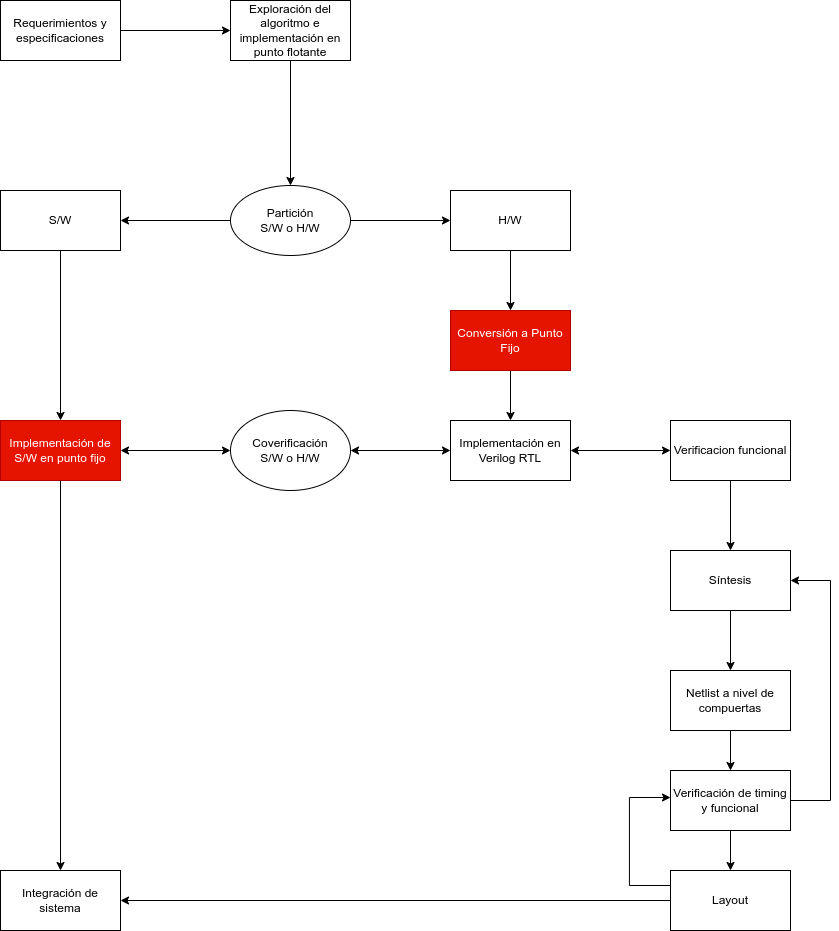
\includegraphics[width=0.8\textwidth]{figures/2.png}
  \caption{\label{fig:fig2}Flujo típico de diseño de sistema en punto fijo}
\end{figure}
Para la implementación del firmware se utiliza la metodología TDD (\textit{Test Driven Development}), que como lo indican sus siglas se basa en el desarrollo guiado por pruebas, y se encuentra ampliamente difundido en la actualidad en el mundo del software embebido. En la Figura \ref{fig:fig3} observamos el ciclo de desarrollo típico de esta metodología. Son numerosas las ventajas de esta decisión de diseño, pero la principal es que al ser el primordial objetivo conseguir un firmware de nivel industrial que se destaque por su robustez y flexibilidad, es esencial conseguir un nivel de \textit{coverage} del 100\%.

\begin{figure}[ht]
  \centering
  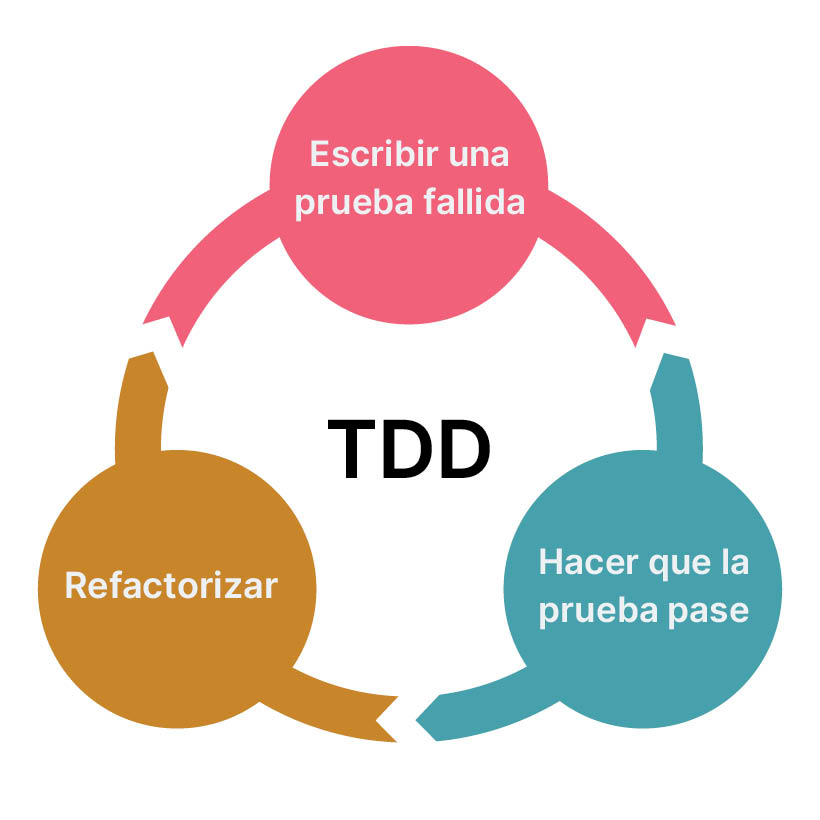
\includegraphics[width=1\textwidth]{figures/3.jpg}
  \caption{\label{fig:fig3}Desarrollo guiado por pruebas}
\end{figure}


 El framework de TDD elegido para desarrollar el código es \textit{Ceedling}, pensado para desarrollar firmware para embebidos en ANSI C, lo cual es parte del proyecto. Para la administración del proyecto se hará uso de la herramienta \textit{Org Mode + Projectile}, que permitirá controlar el cumplimiento de los plazos establecidos en la Planificación (Ver Sección \ref{sec:etapas} ).
\par Por ultimo recalcar que para la programación de la placa de desarrollo, es decir del FPGA se hará uso del software provisto por el fabricante Libero\textregistered, y para la programación del sistema de microprocesadores se hará uso de otro software del fabricante llamado Softconsole\textregistered.
%%% Local Variables:
%%% mode: LaTeX
%%% TeX-master: "../anteproyecto"
%%% End:




%Factibilidad técnica y económica

\section{Factibilidad}
\label{sec:factibilidad}

\subsection{Recursos materiales}
\label{sec:recursos-materiales}

\begin{itemize}
\item Computadora
\item Placa de desarrollo Polarfire Discovery Kit
\item \textbf{Software}: Ceedling, ANSI C, Emacs, Org-Mode, SoftConsole\textregistered, Libero SoC\textregistered.
\end{itemize}

\subsection{Recursos económicos}
\label{sec:recursos-economicos}

\begin{itemize}
\item Precio de la placa de desarrollo Discovery Kit: 132U\$D
\end{itemize}

\vspace{0.5  cm}\par Vale aclarar que el precio de las herramientas de software es cero, debido a que se priorizó la utilización de software libre y código abierto para el desarrollo del mismo, incluyendo las herramientas brindadas por el fabricante de la placa.

%%% Local Variables:
%%% mode: LaTeX
%%% TeX-master: "../anteproyecto"
%%% End:


%Descripción de las etapas del proyecto

\section{Etapas del proyecto}
\label{sec:etapas}
En la figura \ref{fig:fig4} se muestran las distintas etapas del proyecto a realizar, diferenciando claramente las mismas y las tareas que componen a cada una de ellas.
\begin{figure}[ht]
  \centering
  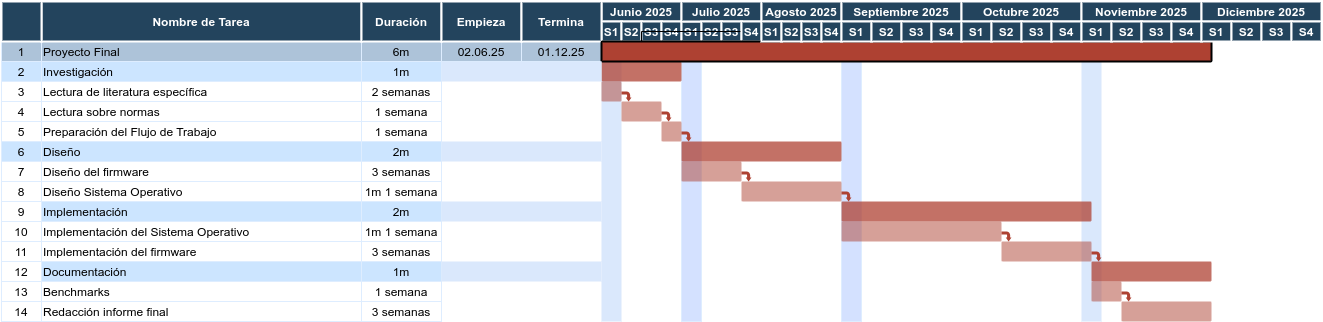
\includegraphics[width=1\textwidth]{figures/4.png}
  \caption{\label{fig:fig4}Planificación del proyecto}
\end{figure}

\pagebreak
\newpage

\begin{enumerate}
\item Se da inicio al proyecto.
\item La etapa de investigación consistirá de la búsqueda y lectura de la literatura especifica del tema, como lo es \cite{De_Vleeschauwer_2017}, con el fin principalmente de poder definir claramente las especificaciones del proyecto.
\item Luego se procede a la lectura y comprensión de la norma vigente para MPEG-2 (ISO/IEC) como se detalla en la bibliografía.
\item Finalmente en esta etapa de investigación incluimos la preparación del flujo de trabajo descrito en la Sección \ref{sec:metodologia}.
\item Pasando ya a la etapa de diseño corresponde comenzar con el dimensionamiento y la arquitectura del firmware, es decir proceder con la maqueta de las tareas de control y monitoreo, y estructura del archivo de registros de configuración, así como la definición de las interfaces y de la estructura en si de la API.
\item Una vez definido el firmware, resulta mas fácil delimitar el tamaño y funcionalidades del sistema operativo, que a priori por tratarse de un sistema en hardware, se tratará de un sistema operativo en tiempo real. Resulta conveniente realizarlo de esta manera para así no cometer errores de sobre diseño para con el sistema operativo.
\item Pasamos a la etapa de implementación, donde ahora se invierte la lógica pues resulta impráctico implementar el firmware sin un sistema operativo que servirá de plataforma cuando vayamos al chip en la vida real. Aquí entonces se realiza una implementación del sistema operativo en tiempo real para un subsistema de 4 microprocesadores RISC-V.
\item Ahora si procedemos con la implementación de las tareas propias del firmware con sus respectiva documentación técnica.
\item Pasamos a la etapa final de documentación. En primer lugar se ejecutarán distintos benchmarks para poder contrastar no solo la performance de nuestro sistema sino también de cada componente, es decir compararemos nuestro sistema operativo con otros comerciales o de amplia difusión, con un propósito más general.
\item Finalmente se dedicarán 3 semanas a la redacción del informe final que ha de ser presentado para la presentación del Proyecto Final.
\end{enumerate}
%%% Local Variables:
%%% mode: LaTeX
%%% TeX-master: "../anteproyecto"
%%% End:
  

\pagebreak
\newpage
 
\nocite{*}
\bibliography{bibliografia}


\listoffigures

\end{document}
%%% Local Variables:
%%% mode: LaTeX
%%% TeX-master: t
%%% End:

